This chapter explains concepts and mathematical theory used in this thesis. First, some mathematical background on procedural texturing in general is presented, followed by the basics of our central algorithm gradient descent, used for parameter estimation, in sections \ref{sec:Gradient} and \ref{sec:StochasticGradientDescent}. In section \ref{sec:AutomaticDifferentiation} the concepts behind automatic differentiation that enables us to develop a differentiable renderer are described. Finally, some related work from different sub-fields of inverse rendering are presented and discussed, illustrating why their solutions were not used in this project.


\section{Procedural Textures}\label{sec:BackgroundProceduralTextures}

Texturing is a method of adding more detail and realism to a 3D object, traditionally by projecting a 2D bitmap texture onto its surface. This is a rather straightforward process, but presents a number of practical problems that are difficult to overcome. Firstly, a bitmap texture has a fixed amount of detail; a pixel resolution. The resolution of an image can normally not be scaled up, although new research has made progress in that aspect much thanks to the advances in neural networks \cite{richard_2019_learned, li_2019_a}. However, even if the resolution is sufficient, bitmap textures are still inflexible as it is difficult to modify the underlying patterns without negatively affecting its overall appearance. Furthermore, bitmap textures require a considerable amount of storage space, especially at high resolutions. Another hurdle that is often overlooked, is the inherent problem of smoothly projecting 2D texture coordinates $p_{2D} = (u,v)$ onto points on a 3D object's surface $p_{3D} = (x,y,z)$. This mapping process is a function from two-dimensional coordinates in a texture matrix to three-dimensional points on an object's surface and is often referred to as \textit{UV mapping}, see equation \ref{eq:UVMapping}, and can give rise to visible seams on the edges between object surfaces as demonstrated in Figure \ref{fig:BitmapVsProcedural}. 

\begin{equation}\label{eq:UVMapping}
    f(u,v) : \mathbb{N}^2 \mapsto \mathbb{R}^3
\end{equation}

Procedural textures, often referred to as \textit{shaders} in computer graphics, are created using mathematical functions that take the surface coordinates of the 3D object as input, as well as a set of $n$ parameters $\theta \in \mathbb{R}^n$ describing its appearance, and returns a color for the point $p_{3D} = (x,y,z)$ see equation \ref{eq:ProceduralMapping}. The parameters $\theta$ can be adjusted by the user to change the underlying patterns and colors, making them much more flexible than the static bitmap approach. They are however slower than conventional bitmap textures as the mathematical functions have to be called thousands of times, once for each pixel, whereas for bitmap textures these values are pre-computed and read into memory. Procedural texturing is therefore mostly used in offline rendering as it introduces too much overhead in real-time rendering.

\begin{equation}\label{eq:ProceduralMapping}
    f(x,y,z,\theta): \mathbb{R}^3, \mathbb{R}^n \mapsto \mathbb{R}^3
\end{equation}


\subsection{Function Composition}

As procedural textures are mathematical functions, their versatility can be extended using \textit{function composition}, a basic mathematical operation taking two functions $f(x)$ and $g(x)$ as input, producing a new function $h(x) = f(g(x))$. While the final output of the procedural texture function should be the color of a point on a target object's surface, any output of any function $g(x)$ can be used as input to a procedural function $f(x)$. To understand how powerful function composition is when used with procedural textures, let $f(\vec{v}, \vec{w}, a)$ be a function of two vectors and a scalar mix factor that returns a weighted sum of both vectors, essentially mixing them. Let $g(x,y,z,a)$ be a function that returns an arbitrary sinusoidal pattern that depends on the input coordinates $(x,y,z)$ as well as a scaling factor $a$ and finally, let $r(x,y,z,\vec{\theta})$ be the main procedural texture function that is a composition of $f$ and $g$. We also define a red color vector and a green color vector, $c_r = (1.0,0.0,0.0)$ and $c_g = (0.0,0.3,0.0)$ where the elements represent the red, green and blue channels. The functions are defined in equation \ref{eq:ProceduralFunctionComposition} where all operators are applied element-wise.

\begin{equation}\label{eq:ProceduralFunctionComposition}
\begin{aligned}
    f(\vec{v}, \vec{w}, a) &= \vec{v} \cdot (1 - a) + \vec{w} \cdot a \\
    g(x,y,z,a) &= \sin(a \cdot x)\cdot \sin(a \cdot y)\cdot \sin(a \cdot z)  \\
    r(x,y,z,\vec{\theta}) &= f(c_r, c_g, g(x,y,z,\theta_0))
\end{aligned}
\end{equation}

We can now texture a plane by coloring each pixel with coordinates $(x,y,z)$, where $z=1$ is constant, with the output of our procedural function $r$, and achieve the result in Figure \ref{fig:ProceduralTextureCompositionPattern}, where parameter $\theta_0$ is set to $20$. Essentially, this procedural strawberry pattern is achieved by mixing the red and green color in function $f$ using the return value of the sinusoidal function $g$ as a factor. Note that the coordinates $0.0 \leq x,y,z \leq 1.0$ are normalized, meaning the pattern is independent of the size of the rendered plane. Refer to appendix \ref{sec:AppendixLinkToStrawberryPatternAtShadertoy} for an online version.

\begin{figure}[!h]
    \centering
    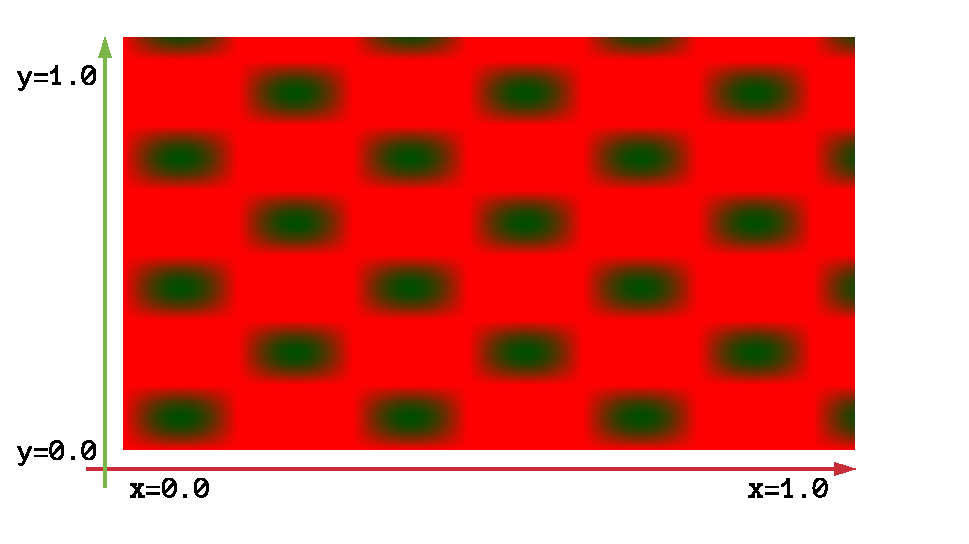
\includegraphics[width=0.7\textwidth]{img/background/Procedural Strawberry Pattern.pdf}
    \caption{Simple procedural strawberry pattern created from composing two functions. The axes show the normalized plane coordinates.}
    \label{fig:ProceduralTextureCompositionPattern}
\end{figure}


\subsection{Procedural Noise}

The real world is full of seemingly unpredictable patterns from the way trees branch out to the uneven surface of a rock. To mimic these patterns in procedural texturing, a type of controlled randomness called noise is extensively used. Noise is deterministic, which means that for the same parameters, a noise function will always generate the same value. Noise also has the property that it is smooth, so that local changes are small and gradual but on a global scale, it looks random. The most famous type of noise is \textit{Perlin noise}, an award winning noise algorithm developed by Ken Perlin in order to create more realistic textures for the movie Tron (1982), formerly described in his paper in 1985 \cite{perlin_1985_an}. The way this and many other noise algorithms generate a pseudorandom, deterministic number from a coordinate $(x,y)$ is by taking the fractional part of a sinusoid that is multiplied by any large number, like shown in equation \ref{eq:Pseudorandom}. This results in a well behaved function that returns a number between $0$ and $1$ that is perceived as random for a relatively large change in coordinate $(x,y)$, but is deterministic. 

\begin{equation}
    rand(x,y) = \fract(\sin(123.23x + 923.1y) \cdot 465123.97)
    \label{eq:Pseudorandom}
\end{equation}

To create smooth 2D noise, Perlin had the idea of smoothly interpolating between four corners of a square, with a pseudorandom value assigned to each corner. If we texture a plane with normalized coordinates using this technique, it will mostly look like a gradient. However, if we simply scale up the coordinates, effectively scaling down the pattern, it will be pseudorandomly repeated across the plane. The pattern will still look rather blocky, and to create an appealing noise pattern, we can utilize what is called \textit{fractal brownian motion}, where any number of octaves of this sinusoidal noise is added with diminishing scale and amplitude. The progress towards a deterministic cloud pattern is shown in Figure \ref{fig:ProceduralNoise}. 

\begin{figure}[!h]
    \centering
    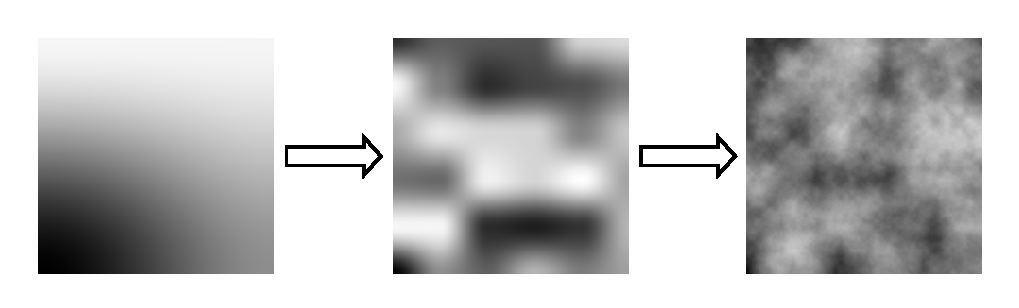
\includegraphics[width=1.0\textwidth]{img/background/Procedural Noise.pdf}
    \caption{Left: Perlin noise interpolated between four corners of a plane. Middle: The normalized coordinates of this plane can be scaled up, in this example five times, to add more detail. Right: Finally, to achieve a cloud pattern, octaves of the noise is summed using different scale values and amplitudes.}
    \label{fig:ProceduralNoise}
\end{figure}

\section{Gradient}\label{sec:Gradient}

A concept commonly used throughout this thesis is the \textit{gradient} of a function, which is a generalization of the ordinary derivative. Indeed, the gradient of a function $f(x)$ of a single variable is equal to the derivative of $f$ with respect to $x$, denoted $\frac{d f}{d x}$. For a multivariate function $f(x_1, x_2, \dots, x_n)$ however, the gradient of $f$, denoted $\nabla f$, is defined as the vector of partial derivatives of $f$ with respect to each argument, as shown in equation \ref{eq:GradientDef}.

\begin{equation}\label{eq:GradientDef}
    \nabla f(x_1, x_2, \dots, x_n) = \begin{bmatrix} \frac{\partial f}{\partial x_1} & \frac{\partial f}{\partial x_2} & \dots & \frac{\partial f}{\partial x_n} \end{bmatrix}
\end{equation}

The derivative famously describes a function's rate of change, or direction of greatest increase. Similarly, for a multivariate function $f$ of $n$ variables, the gradient is an $n$ dimensional vector in the direction of greatest increase, also called the direction of \textit{steepest ascent}. This stems from the common depiction of multivariate functions as surface plots with the gradient pointing in the direction where the surface has the steepest upward slope. In minimization problems, the gradient can be used to find the direction of \textit{steepest descent}, which is simply defined as the negative of the gradient \cite{faul_2020_a}.




% \subsection{Vector-Jacobian product}
% The PyTorch operators accept Tensors of arbitrary shape, and so the general case, we want to find the gradient of a \textit{vector valued} function. Given a function $\vec{y} = f(\vec{x})$ where $\vec{x}=(x_0,x_1,...,x_n)$ and $\vec{y} = (y_0,y_1,...,y_m)$ the gradient of $f$ is a so called \textit{Jacobian Matrix}, which is a matrix of all possible partial derivatives of the two vectors $\vec{x}$ and $\vec{y}$, see equation \ref{eq:JacobianMatrix}.

% \begin{equation}\label{eq:JacobianMatrix}
%     \nabla f = J = 
%     \begin{bmatrix} \frac{\partial y_0}{\partial x_0} & \frac{\partial y_0}{\partial x_0} & \dots & \frac{\partial y_0}{\partial x_n} \\ 
%     \frac{\partial y_1}{\partial x_0} & \frac{\partial y_1}{\partial x_1} & \dots & \frac{\partial y_1}{\partial x_n} \\
%     \vdots & \vdots & \ddots & \vdots \\ 
%     \frac{\partial y_m}{\partial x_0} & \frac{\partial y_m}{\partial x_n} & \dots & \frac{\partial y_m}{\partial x_n}
%     \end{bmatrix}
% \end{equation}

% The vector-Jacobian product is the product of a vector $v=(v_0,v_1...v_n)$ and the Jacobian matrix $v^T \cdot J$ and generally, the \texttt{autograd} package of PyTorch is an engine for computing this product.

% Going back to figure \ref{fig:ComputationalGraph}, we call the multiplication operator $mul$ and the addition operator $add$.  We can rewrite rewrite our mathematical notation of $d=(a+b)*3$ in a more programmatical syntax \codeinline[]{d = mul(add(a,b),3)}. To calculate the derivative of $d$, we use the chain rule as shown in equation \ref{}

% \begin{equation}\label{eq:ChainRuleExample}
%     \begin{aligned}
%     \frac{d}{d}mul(add(a,b),3) = \frac{d mul}{d add} \prod \frac{d add}{}
%     \end{aligned}
% \end{equation}

% \textbf{CITE autograd!} \cite{autograd}

\section{Stochastic Gradient Descent}\label{sec:StochasticGradientDescent}

The gradient descent algorithm is one of the cornerstones of this project and is in fact a fairly simple algorithm for iteratively optimizing a, most often, multivariate function. It is a popular algorithm in machine learning where it is used to minimize the loss of a neural network model as measured by a loss function. It works by iteratively finding the direction of steepest descent of the loss function defined as the negative of a function's gradient, as explained in section \ref{sec:Gradient}, eventually leading to a minimal loss value. Finding the gradient of a complex function can be done automatically and reliably if defined in an automatic differentiation framework as explained in section \ref{sec:AutomaticDifferentiation}. 

There are a few major versions of the gradient descent algorithm, the most commonly used in machine learning being mini-batch gradient descent, where the gradient is calculated as an average of multiple samples in order to complete a single step or iteration. Stochastic gradient descent on the other hand, performs one step for each sample, which is used in our implementation as we only have a single sample (a user's input image). The general algorithm of gradient descent is presented in pseudo-code in Algorithm \ref{alg:GradientDescent}. Starting with an arbitrary parameter vector $\theta \in \mathbb{R}^n$ which contains all $n$ parameters needed to define an output procedural texture, as well as a loss function $\mathcal{L}$ with $\nabla \mathcal{L}(\theta)$ denoting the gradient of $\mathcal{L}$ with respect to each parameter in $\theta$, we can update our parameters in each iteration $t$ as shown in equation \ref{eq:GradientDescentUpdate}

\begin{equation}\label{eq:GradientDescentUpdate}
    \begin{aligned}
    v_t = \alpha \cdot \nabla \mathcal{L}(\theta_t) \\
    \theta_{t+1} = \theta_t - v_t
    \end{aligned}
\end{equation}

The variable $\alpha \in [0,1]$ is called the learning rate and controls how fast $\theta$ will converge toward the optimal parameter set $\theta^*$ that minimizes our loss function $\mathcal{L}$. The strategy for updating the parameters can be refined by using a different \textit{Optimizer}, see section \ref{sec:Optimizer}. As we will see in section \ref{sec:LossFunctions}, loss functions generally don't depend directly on the parameters in $\theta$, but instead on two values, a target and a sample which are generated using $\theta$. 

% \begin{equation}\label{eq:GradientDescentOptimization}
%     \argmin_{\theta} \mathcal{L}(\theta) = \left\{\theta \mid \mathcal{L}(\theta) = \min_{\theta^*} \mathcal{L}(\theta^*)\right\}
% \end{equation}

\begin{algorithm}[H]
\SetKwData{L}{loss}\SetKwData{Iter}{iter}\SetKwData{Target}{target}\SetKwData{RenderedImage}{sample}\SetKwData{Theta}{$\theta$}\SetKwData{ThetaOpt}{$\theta^*$}
\SetKwFunction{Loss}{$\mathcal{L}$}\SetKwFunction{Optimize}{Optimize}\SetKwFunction{Compute}{Compute}\SetKwFunction{GradLoss}{$\nabla\mathcal{L}$}
\SetKwInOut{Input}{Input}\SetKwInOut{Output}{output}

\KwResult{Optimal set of parameters \ThetaOpt that minimizes loss function \Loss{$\hat{X}, X$}}
\Input{The loss goal $l_{goal}$, maximum number of iterations $i_{max}$, and a target \Target.}

\BlankLine
Randomly or strategically initialize \Theta\;
\Iter $\leftarrow$ $0$\;
\While{\Iter $<$ $i_{max}$}{
    \RenderedImage $\leftarrow$ \Compute{\Theta}\;
    \L $\leftarrow$ \Loss{\RenderedImage, \Target} \;
    \If{\L $\leq$ $l_{goal}$}{
        \Return \Theta\;
    }
    Backpropagate \L to find the gradient \GradLoss w.r.t \Theta\;
    $\theta\leftarrow$\Optimize{\Theta, \GradLoss} \tcc*[r]{Update \Theta according to optimizer}
    \Iter $\leftarrow$ \Iter $+1$\;
}
\Return \Theta\;
\caption{Stochastic Gradient Descent Algorithm}\label{alg:GradientDescent}
\end{algorithm}


\subsection{Optimizers}\label{sec:Optimizer}

Optimizers are algorithms describing a strategy for gradient descent to reliably reach the most optimal value of the loss function in the least number of steps possible. This is achieved by controlling the updating of the parameters in such a way that the largest steps possible are taken towards the optimal loss value, without overshooting it or getting stuck in local minima. An analogy often used to describe an optimizer's progress is that of a ball rolling towards the lowest point on a surface (the loss function) in the direction of the downward slope (steepest descent). Given a loss function $\mathcal{L}$, the most basic optimizer updates each parameter in $\theta$ according to equation \ref{eq:GradientDescentUpdate} shown earlier. Additionally, for each iteration $t$, the learning rate is usually updated by multiplying it with a decay term $\delta$ so that it diminishes over time. This is to prevent it from overshooting the minimum by forcing it to take smaller steps the closer it gets to the minimum. The drawback of this simple solution is that it is not very adaptive, and uses the same learning rate for all parameters, and will thus give us problems when the derivative differs between parameters. To overcome this, optimizers usually implement something called \textit{momentum}, which adds a fraction $0 \leq \beta \leq 1$ of past update vectors to the current update vector $v_t$. The update steps now become:

\begin{equation}
    \begin{aligned}
    v_t = \beta v_{t-1} + \alpha \cdot \nabla \mathcal{L}(\theta) \\
    \theta_{t+1} = \theta_t - v_t
    \end{aligned}
\end{equation}

This is effectively an exponentially weighted moving average, and for parameters where the gradient is oscillating, this addition will average out those oscillations. However, each parameter in $\theta$ still gets updated using the same learning rate $\alpha$. To correct this, an additional term dubbed \textit{second moment} is calculated, which is a squared weighted average of the past gradients, popularized by \textit{Adagrad} \cite{duchi_2011_adaptive} and refined in \textit{Adadelta} \cite{zeiler_2012_adadelta}. The combination of momentum (first moment) and second moment is used in \textit{Adam} or \textit{Adaptive Moment Estimation}, one of the most popular and successful optimization algorithms used in machine learning \cite{kingma_2014_adam}. The first and second moments, $m_t$ and $v_t$, for an iteration $t$ are calculated in equation \ref{eq:FirstSecondMoment}.

\begin{equation}\label{eq:FirstSecondMoment}
    \begin{aligned}
    m_t = \beta_1 m_{t-1} + (1-\beta_1) \cdot \nabla \mathcal{L}(\theta) \\
    v_t = \beta_2 v_{t-1} + (1 - \beta_2) \cdot \nabla \mathcal{L}(\theta)^2
    \end{aligned}
\end{equation}

The two parameters $0 \leq \beta_1, \beta_2 \leq 1$ are used to tune how fast the influence of previous iterations should decay, and is recommended by the authors to be set to $\beta_1 = 0.9$ and $\beta_2 = 0.999$. The second moment, which is a running average of the square of the gradients, controls how much influence the learning rate $\alpha$ has on each parameter in $\theta$, as shown in equation \ref{eq:Adam}.

\begin{equation}\label{eq:Adam}
    \theta_{t+1} = \theta_t - \frac{\alpha}{\sqrt{v_t} + \epsilon}m_t
\end{equation}

The $\epsilon$ is a small corrective term to prevent division by zero errors. Note that all variables, except $\epsilon$ and $\alpha$ are vectors of size $n$, the number of parameters in $\theta$ and all operations are performed element-wise. Before the first iteration, $m_t$ and $v_t$ are initialized to all zeros, which introduces a bias towards zero for the early iterations. To prevent this, $m_t$ and $v_t$ in equation \ref{eq:Adam} are replaced with their bias corrected versions, $\hat{m}_t$ and $\hat{v}_t$, which are calculated in equation \ref{eq:BiasCorrectedMoments}.

\begin{equation}\label{eq:BiasCorrectedMoments}
    \begin{aligned}
    \hat{m}_t = \frac{m_t}{1- \beta_1^t} \\
    \hat{v}_t = \frac{v_t}{1 - \beta_2^t}
    \end{aligned}
\end{equation}

As the iteration counter $t$ increases, the denominator $1 - \beta^t$ converges towards $1$ and will thus have a negligible effect on the moments in later iterations. Most other optimizers build on these concepts.

\subsection{Loss Functions}\label{sec:LossFunctions}

Gradient descent is commonly used to minimize a function that measures the difference between a generated sample $\hat{X}$, our prediction, and a ground truth $X$, the target, as a single real number. Such a function is often referred to as a \textit{loss function} or \textit{cost function} as it represents a penalty that we desire to be as small as possible. In our case, we can use it to measure the difference between a user input texture image, our target, and an image that our system has generated. A loss function should conventionally output a single scalar value, where larger values represent a bigger difference and a value of zero represents two identical images, at least as measured by the loss function. In theory, an image loss function could have any input, but the convention is shown in equation \ref{eq:LossFunctionMapping}, where $\mathcal{L}$ denotes a loss function that maps an input of two image matrices $\hat{X}$ and $X$ to a real scalar value. The matrices are real valued and in \textit{column-first} order which is why the width is specified first in $\mathbb{R}^{w \times h \times 3}$, where $w$ and $h$ is the width and height of a rendered image with three color channels.

\begin{equation}
    \begin{aligned}
    \mathcal{L}: \hat{X},X \mapsto \mathbb{R} \\
    \text{where } \hat{X}, X \in \mathbb{R}^{w\times h \times 3} \text{ and } w, h \in \mathbb{N}
    \end{aligned}
    \label{eq:LossFunctionMapping}
\end{equation}

The choice of loss function fully depends on what is being measured. Loss functions for images are a special case and often it is desirable to design it in a way that coincides with humans' perceived difference of two images, which can be difficult as the human visual system is very complex. Often simple functions like Mean Squared Error, explained below, are very sensitive to spatial changes in data, which is why more advanced functions are often required.

\subsubsection{Mean Squared Error}\label{sec:MeanSquaredError}

Mean Squared Error is a popular and simple loss function that, when used on images, measures the squared difference of each pixel, sums them and returns the mean of the sum as shown in equation \ref{eq:MSE}. This kind of loss function is useful if the goal is to reproduce the target image down to the pixel. This is however, not a good representation of how a human would judge the similarity of two images. If target image $X$ and predicted image $\hat{X}$ are identical, except each pixel in $\hat{X}$ is shifted one column to the right, it would still be very hard to distinguish any difference between the two for a human (given a reasonable resolution). However, depending on the amount of noise in the image, most pixels are no longer identical and a large difference is measured. This also applies to any scaling, rotation or sheering of images and thus MSE has a strong spatial dependency on the compared images. Especially for procedural texturing, where high frequency features and patterns are common, we need to look for more sophisticated means of measuring differences between images.

\begin{equation}\label{eq:MSE}
    \mathcal{L}_{MSE}(\hat{X}, X) = \frac{1}{w\cdot h\cdot 3}\sum_{i,j,c} (\hat{X}_{i,j,c} - X_{i,j,c})^2
\end{equation}

\subsubsection{Neural Feature Loss}\label{sec:NeuralFeatureLoss}

Developing a reliable method of measuring differences in images is important in inverse graphics as well as machine learning and directly affects its performance. In a way, our algorithm is only as good as our loss function which defines an upper bound on accuracy. In the paper by Guo et. al \cite{guo_2019_a}, several different loss functions are discussed, reaching the conclusion that a function utilizing features extracted by a neural network such as VGG19 performed best \cite{simonyan_2015_very}, a method directly adapted from a paper by Gatys et. al. \cite{gatys_2015_texture}. Hu et. al. also used a version of this as the loss function for their neural network model, but calculated histograms on the features instead \cite{hu_2019_a}.

A convolutional neural network like VGG19 contains a series of sequential layers through which a generated image $\hat{X}$ and a target image $X$ are passed. The activations in the layers form so called \textit{feature maps}, a kind of filtered image. Each layer $l$ has $N_l$ filters, each producing one feature map of size $M_l$ when vectorized, which are stored in a feature matrix $F^l \in \mathbb{R}^{N_l \times M_l}$. What we end up with is a set of these feature matrices for each of the two input images. These matrices are flattened to vectors and the dot product is utilized to measure their similarity. The dot product of two vectors is given by the equation \ref{eq:DotProduct}, where a small angle $\theta$ indicates similar vectors. Thus a small value of the dot product between two features maps of the same layer $l$, implies similar features. 

\begin{equation}\label{eq:DotProduct}
    \vec{v} \cdot \vec{w} = \left|v\right|\left|w\right|\cos(\theta) = v_1w_1 + v_2w_2 + \dots v_{M_l}w_{M_l}
\end{equation}

Flattening feature matrices into vectors and computing the dot product between them effectively removes the spatial information in the features. The feature correlations of layer $l$ are given by the so called \textit{Gram matrix} $G^l \in \mathbb{R}^{N_l\times N_l}$, produced by the dot product between the vectors in the two feature matrices as shown in equation \ref{eq:GramMatrix}.

\begin{equation}\label{eq:GramMatrix}
    G^l_{ij} = \sum_k F^l_{ik}F^l_{jk}
\end{equation}

Features can be extracted from any number of layers and collected as a set of Gram matrices $\{G^1, G^2, \dots, G^L\}$. A weighted sum squared error of the set of gram matrices is used to calculate the final loss like shown in equation \ref{eq:NeuralLoss}, where weights $w_l$ are set per layer.

\begin{equation}\label{eq:NeuralLoss}
    \mathcal{\mathcal{L}}(\hat{X},X) = \sum_{l=0}^L\underbrace{\frac{w_l}{4N_l^2M_l^2}\sum_{i,j}\left(G^l_{ij} - \hat{G}^l_{ij}\right)^2}_{\text{weighted contribution per layer }l}
\end{equation}

This type of loss function typically perform well for images and correspond to the human visual system, but is slowed down substantially if layers are selected far from the input, as the images have to be passed through each preceding layer. Using a pre-trained neural network such as VGG19 means we can skip the time consuming and difficult work of training on millions of images, but comes with the disadvantage of requiring input of a specific resolution of $224\times224$ pixels.

\section{Automatic Differentiation}\label{sec:AutomaticDifferentiation}

The rendering process needs to be differentiable in order to be inverted, and is a major reason why inverse rendering is a difficult problem. Why differentiability is a requirement relates to our iterative optimization Algorithm \textit{Gradient Descent}, explained in section \ref{sec:StochasticGradientDescent}, which uses the gradient of a loss function to find the direction where it decreases the most.

The rendering process can be seen as one, very convoluted function of many parameters that completely describe a 3D scene, for which the derivatives with respect to each independent parameter needs to be calculated. This is completely infeasible in almost all modern renderers like those utilized by \textit{Blender} or \textit{3Ds Max}, but can be achieved if fully implemented in a framework that supports \textit{automatic differentiation}.

Automatic Differentiation, usually abbreviated AD or \textit{autograd}, is a method of automatically calculating gradients of functions, specifically functions defined in a programming language. Different libraries implement AD in different ways, but most work by breaking down complex functions into primitive expressions for which the derivative is known and all other, more complex functions, must be created using these building blocks. The order that these primitives are applied to variables is mapped in a \textit{Computational Graph}, which is the main feature of the AD algorithm. 

\subsection{Chain Rule}\label{sec:ChainRule}

As function composition is a natural part of mathematics and any programming language, an automatic differentiation framework needs to be able to handle this. To differentiate a composite function, the \textit{chain rule} is used, which is shown in equation \ref{eq:ChainRule}. This rule states that the derivative of a composite function $h(x) = f(g(x))$ is equal to the product of the derivative of the outer function $f'$ and inner function $g'$. The chain rule is central to the automatic differentiation algorithm which, in a way, is nothing more than a way of recording operations used on a variable and correctly applying the chain rule.

\hl{THE CODE HIGHLIGHTING}
\begin{equation}\label{eq:ChainRule}
    \frac{d f(g(x))}{dx} = \frac{d f}{dg} \times \frac{d g}{d x}
\end{equation}

\subsection{Computational Graph}\label{sec:ComputationalGraph}

There exists a myriad of different automatic differentiation packages today, using different techniques. Common among them is using building blocks of functions with known derivatives as well as recording the order and settings with which these functions are applied to variables in order to correctly apply the chain rule. Often they require the user to define variables using a custom data structure that stores the state and data of the variable, often referred to as a Tensor as they support data of any dimension, be it scalars, vectors or matrices. Popular packages today, like Google's Jax, TensorFlow, or Facebook's PyTorch record computations in a data structure called a computational graph, a directed acyclic graph with nodes corresponding to variables and applied functions.

\begin{codefig}
\begin{minted}{python}
x = Tensor(1.5)
y = Tensor(4.0)
z = mul(x, y)  # x*y = Tensor(6.0)
h = pow(z, 3.0)  # z^3 = Tensor(216.0)
dh_dx = gradient(h, x)  # Tensor(432.0)
\end{minted}
    \caption{Generic example of operations applied to variables and the gradient being calculated.}
    \label{code:CodeComputationalGraph}
\end{codefig}

Code \ref{code:CodeComputationalGraph} shows a general example of operations performed on two variables and the gradient being calculated. The additional intermediate variable $z$ is not strictly needed, but allows for a more informative computational graph. In the code example, the \texttt{gradient} function calculates $\frac{\partial h}{\partial x}$, the derivative of $h$ with respect to $x$. We can do this mathematically by using the chain rule and applying standard derivatives, as shown in equation \ref{eq:CalculatingDerivative} where we have assigned shorthand functions $m(x,y)=x\cdot y$ and $p(x,y)=x^y$ to represent the multiplication and the power operations respectively, making $h(x,y)=p(m(x,y),3.0)$ a composite function of $p$ and $m$.

\begin{equation}\label{eq:CalculatingDerivative}
    \frac{\partial h}{\partial x} = \frac{\partial p}{\partial m} \cdot \frac{\partial m}{\partial x} = \frac{\partial}{\partial m}m^3 \cdot \frac{\partial}{\partial x}(x\cdot y) = 3m^2 \cdot y = 3 \cdot (x \cdot y)^2 \cdot y = 3\cdot (1.5\cdot 4)^2 \cdot 4 = 432
\end{equation}

\begin{figure}[!h]
    \centering
    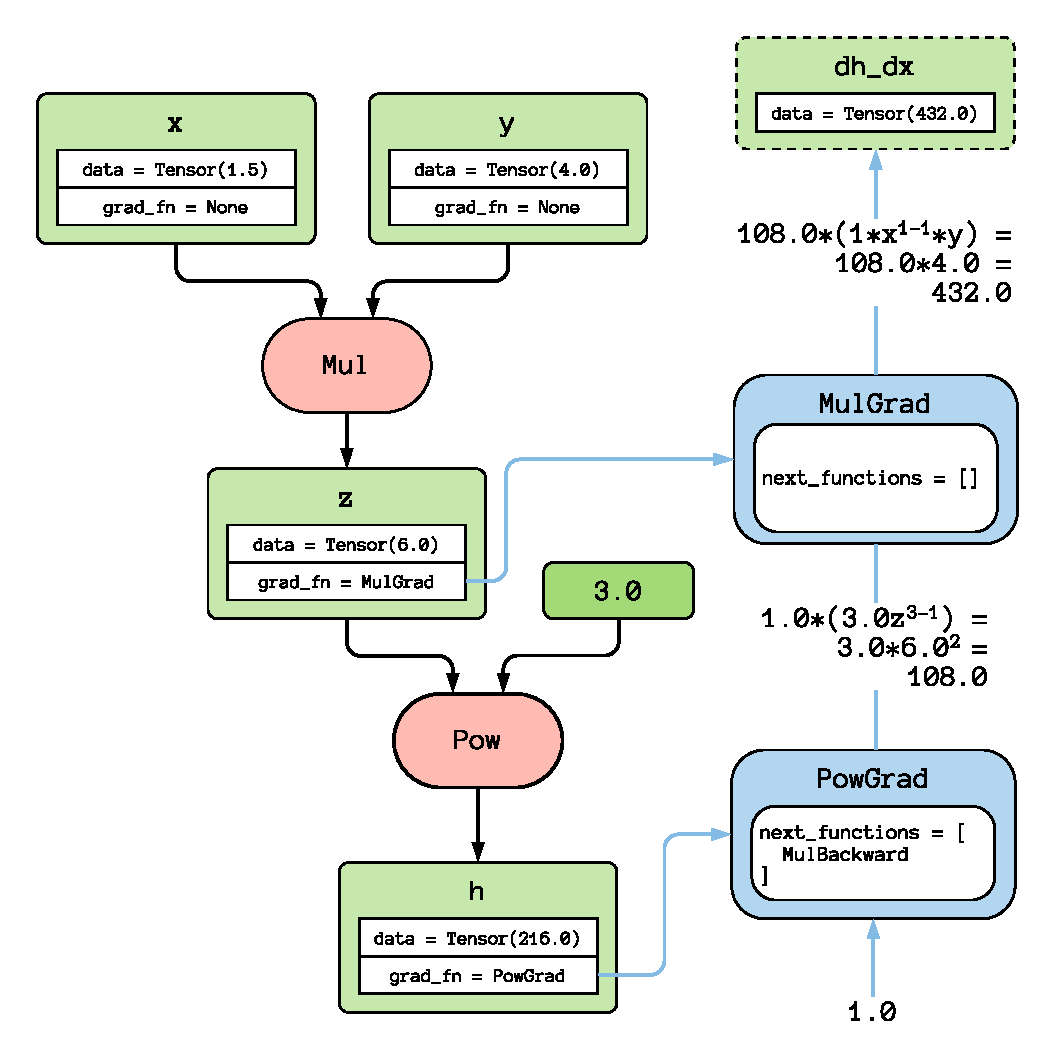
\includegraphics[width=0.8\textwidth]{img/background/Computational Graph.pdf}
    \caption{The computational graph created from the operations in Figure \ref{code:CodeComputationalGraph}. Green nodes represent variables, red nodes operations and blue nodes the backwards operations that calculate gradients.}
    \label{fig:ComputationalGraph}
\end{figure}

In Figure \ref{fig:ComputationalGraph}, the computational graph that is created as a result of the operations in \ref{code:CodeComputationalGraph} is shown. Green nodes represent variables, red nodes represent operations and blue nodes represent the differential version of the operator that calculates the gradient. The variable nodes have a \texttt{data} attribute to track their tensor value and a \texttt{grad\_fn} attribute to track the gradient version of the function that created it. The two variables $x$ and $y$ are connected to the \texttt{Mul} operator node, which outputs a new variable $z$. The new variable $z$, as well as a scalar constant, are connected to the \texttt{Pow} operator which finally results in a new variable $h$. When the gradient is requested the flow backward commences, starting from the target node $h$. Because $h$ was created from function \texttt{Pow}, the next gradient function to evaluate is \texttt{PowGrad} which has internally registered that $z$ and the constant scalar $3.0$ were used as input to \texttt{Pow}. There exists no outer function to evaluate for this gradient, so a value of $1.0$ is used to multiply with the inner gradient according to the chain rule. The output of \texttt{PowGrad} is the gradient of $z$, which is sent to the next gradient function node \texttt{MulGrad}. The inner derivative $\frac{\partial z}{\partial x}$, where $z=x\cdot y$ is evaluated using common derivation rules to $1.0\cdot x^{1-1}y = y$ and is multiplied by the outer gradient from \texttt{PowGrad} according to the chain rule. The returned result $432$ is the gradient of $h$ with respect to $x$. This shows how the computational graph is a powerful tool to calculate gradients of arbitrarily complicated functions with respect to any input variable.

\section{Interpolation}\label{sec:Interpolation}

Interpolation is the mathematical process of estimating new data points withing a range of known data points. It is popularly used in computer graphics because interpolating data is often computationally cheaper than explicitly calculating the new data. Interpolation is a popular tool in animation where an artist can specify key points and let an algorithm smoothly estimate an object's movement in between these points using interpolation. Another popular use case, and one very relevant to this project, is the interpolation of pixel data between known vertex data. In computer graphics, vertices are almost always clustered in groups of three to form triangles and interpolation is performed between these three vertices as in Figure \ref{fig:Interpolation}. Such a triangle $(p_a,p_b,p_c)$ is defined by its three vertices $p_a,p_b,p_c$ and any point $p$ inside this triangle can be expressed as in equation \ref{eq:Interpolation}.

\begin{equation}\label{eq:Interpolation}
    p = a \cdot p_a + b \cdot p_b + c \cdot p_c
\end{equation}

The set $(a,b,c)$ contains the so called \textit{barycentric coordinates} of point $p$ with the restrictions that $a+b+c = 1$ as well as $0 \leq a,b,c \leq 1$. The \textit{barycentric coordinates} act as weights when calculating each vertex's influence on the interpolated value for $p$ and as such, should all sum to $1$, as there can not be more than 100\% total influence at any point in the triangle. From this stems that if a point $p$ is equal to any of the vertices, then the weight for that vertex is $1.0$ and $0.0$ for all other.  Let $A$ denote the area of the triangle $(p_a,p_b,p_c)$, and $A_a$ denote the area of the sub-triangle opposite point $p_a$, then the barycentric coordinate $a = \frac{A_a}{A}$, thus, the barycentric coordinates are essentially the normalized areas of each sub-triangle, as seen in Figure \ref{fig:InterpolationRight}. Using the equation in \ref{eq:Interpolation}, we can calculate any attribute for the fragment shown in Figure \ref{fig:InterpolationRight} by interpolating attributes from $p_a$,$p_b$ and $p_c$. The trigonometry required to actually calculate the areas of the triangles is not relevant to understanding interpolation at this point, so we can assume plausible values for $a$, $b$ and $c$.

\begin{equation*}
    \begin{aligned}
    \text{let } a = 0.6 \text{, } b = 0.15 \text{ and } c = 0.25\\
    a + b + c = 0.6 + 0.15 + 0.25 = 1
    \end{aligned}
\end{equation*}

We verify that all weights sum to one and lie in the interval $[0,1]$. It is now straight forward to find the interpolated value of any attribute, for example the coordinate, of the fragment $f$, calculated from its center point $p_f$ as seen in equation \ref{eq:InterpolatingCoordinate}.

\begin{equation}\label{eq:InterpolatingCoordinate}
    \begin{aligned}
        p_f = 0.6 \cdot (0,0,0) + 0.15 \cdot (1,0,0) + 0.25\cdot (1,1,0) \\
        = (0+0.15+0.25, 0+0+0.25, 0+0+0) \\
        = (0.4, 0.25, 0)
    \end{aligned}
\end{equation}

% Any input attributes to the fragment shader (declared using the \codeinline[glsl]{in} keyword) are interpolated between vertices before being sent to the fragment shader. It is important to notice that vertices may not only contain a position, but other arbitrary data referred to as \textit{attributes}, which also get interpolated. In this way, its possible to provide the fragment shader with normalized fragment positions as long as the position is set in the vertex shader. This special variable is extensively used in our shaders and will be referred to as  \codeinline[python]{frag_pos} and is a vector on the form $(x,y,z)$ where $x,y,z \in [0,1]$. Having a normalized fragment position means that no matter how our object is shaped, every position on its surface is defined in the range $[0,1]$ where a value of $1.0$ identifies the maximum point on that object in a specific direction. As explained in section \ref{sec:CoordinateSystem}, a user can define the vertices in any arbitrary coordinate system, as long as they are normalized in the vertex shader. To do this, the maximum and minimum values of the user defined coordinate system are needed as input to the vertex shader. The attribute \codeinline[glsl]{frag_pos} is calculated as $frag\_pos = \frac{in\_vert\_pos - mins}{maxes-mins}$. After the rasterizer has calculated which fragments belong to which triangle, the vertex attributes are interpolated. A triangle $(p_a,p_b,p_c)$ is defined by its three vertices $p_a,p_b,p_c$ and any point $p$ inside this triangle can be expressed as in equation \ref{eq:Interpolation}.

% \begin{equation}\label{eq:Interpolation}
%     p = a \cdot p_a + b \cdot p_b + c \cdot p_c
% \end{equation}

% We have assumed plausible values for the different weights or normalized areas and verified that they all sum to one. It is now straight forward to find the interpolated value of any attribute for the fragment $f$, calculated from the center point $p_f$ as.

% In equation \ref{eq:Interpolation}, $(a,b,c)$ are the so called \textit{barycentric coordinates} of the point $p$ with the restrictions that $a+b+c = 1$ as well as $a,b,c \in [0,1]$. The \textit{barycentric coordinates} act as weights when calculating each vertex's influence on the interpolated value for $p$ and as such, should all sum to $1$, as there can not be more than 100\% total influence at any point in the triangle. From this stems that if a point $p$ is equal to any of the vertices, then the weight for that vertex is $1.0$ and $0.0$ for all other. The barycentric coordinates are essentially the normalized areas of each sub-triangle. Let $A$ denote the area of the triangle $(p_a,p_b,p_c)$, and $A_a$ denote the area of the sub-triangle opposite point $p_a$, then the barycentric coordinate $a = \frac{A_a}{A}$. Using the equation in \ref{eq:Interpolation}, we can calculate the attribute \codeinline[glsl]{frag_pos} for the fragment shown in figure \ref{fig:InterpolationRight} if we assume values for $a$,$b$ and $c$.

% \begin{equation*}
%     \begin{aligned}
%     \text{let } a = 0.6 \text{, } b = 0.15 \text{ and } c = 0.25\\
%     a + b + c = 0.6 + 0.15 + 0.25 = 1
%     \end{aligned}
% \end{equation*}

% For the sake of argument we have assumed plausible values for the different weights and verify that they all sum to one. Exactly how the areas are calculated in OpenGL is not important. It is now very straight forward to find the interpolated value of any attribute for the fragment $f$, calculated from the center point $p_f$.

% \begin{equation*}
%     \begin{aligned}
%         p_f = 0.6 \cdot (0,0,0) + 0.15 \cdot (1,0,0) + 0.25\cdot (1,1,0) \\
%         = (0+0.15+0.25, 0+0+0.25, 0+0+0) \\
%         = (0.4, 0.25, 0)
%     \end{aligned}
% \end{equation*}

\begin{figure}[h]
\centering
\begin{subfigure}{.4\textwidth}
    \centering
    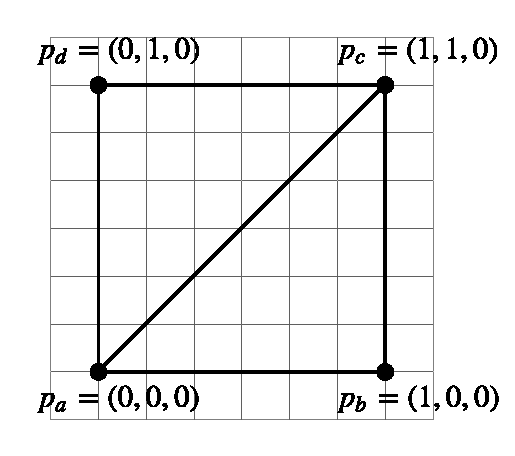
\includegraphics[width=\linewidth]{img/background/InterpolationLeft.pdf}
    \caption{A plane in 3D space with each vertex's coordinate displayed.}
    \label{fig:InterpolationLeft}
\end{subfigure}\hspace{0.6cm}
\begin{subfigure}{.4\textwidth}
    \centering
    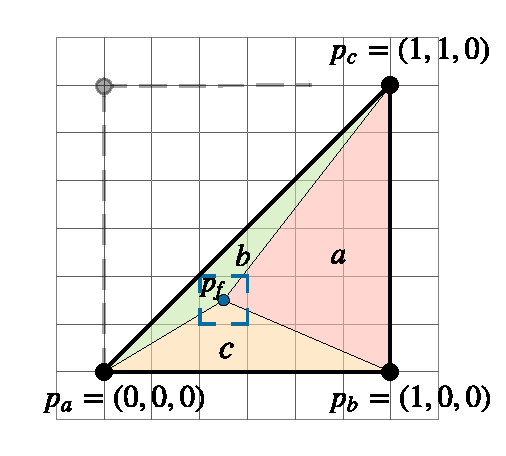
\includegraphics[width=\linewidth]{img/background/InterpolationRight.pdf}
    \caption{Interpolation of a point $p_f$ inside a triangle in the plane.}
    \label{fig:InterpolationRight}
\end{subfigure}
\caption{
Interpolation of vertex coordinates between the three vertices of a triangle for a fragment at point $p_f$ inside the triangle. A weight $w \in \{a,b,c\}$ is equal to the normalized area of the triangle opposite the vertex $p_w$.
}
\label{fig:Interpolation}
\end{figure}


\section{Inverse Graphics}\label{sec:BackgroundInverseGraphics}
Inverse graphics is a broad subject that encompasses much more than just 2D texture acquisition. Many techniques for solving these problems have been developed, some closely related to this project and others completely different but with a similar goal. We have already discussed a few forms of inverse graphics and even tested some during this project but in order to gain a more complete understanding of our work, some of these will be reviewed from an inverse procedural texturing perspective.

\subsection{Inverse Graphics using Neural Networks}

A popular approach to the inverse graphics problem is to use neural networks. Kulkarni et. al propose using a modified Variational Auto Encoder to learn disentangled 3D transformation properties (such as rotation about an axis, or the azimuth of the light source) of a 3D scene \cite{kulkarni_2015_deep}. A \textit{disentangled} representation means that each latent variable $z_i$ in the VAE represents a distinct and isolated transformation of the 3D scene. This is achieved, in part, by training on batches of images where all but one parameter are kept constant. A similar approach is used in a paper by Mahendran et. al, although using a convolutional neural network \cite{mahendran_2017_3d} while a third solution is to use a Generative Adversarial Network that imitates a graphics renderer, which Shi et. al recently proposed to retrieve parameters for 3D faces from 2D images \cite{shi_2019_facetoparameter}. Neither of these solutions specialize in inverse rendering of textures, but instead focus on a small subset of possible 3D scene parameters or in the case of Shi et. al. a pre-defined set of 3D face parameters. This approach can be adapted for simple pre-defined procedural textures, but is difficult to train on more complex examples. Neural networks also require a lot of preparation, such as generating training data which in turn requires pre-designed texture models and are therefore not a flexible solution.

\subsection{SVBRDF Aquisition}

SVBRDF acquisition is a popular subdivision of inverse graphics for textures that aims to decompose 2D image textures into spatially-varying bi-directional reflectance distribution functions maps (SVBRDF for short), a type of image data that describes a texture's roughness, specularity or 3D displacement (normal map) etc. Many papers have in recent years used different neural network models or image analysis to achieve this \cite{deschaintre_2018_singleimage, kang_2018_efficient, nalbach_2017_deep, aittala_2016_reflectance}. However, instead of finding these maps directly, our thesis focuses on finding the parameters to a procedural texture model that would allows us to theoretically generate these maps if necessary, although we do not consider any 3D displacement or light interaction in \dipter{}.

\subsection{Texture Synthesis}

Texture synthesis is a very active research area where a sample image is used to generate a larger texture with the same pattern and style. Virtually all texture synthesis solutions work with bitmap textures, and thus act as an alternative solution to procedural textures when the goal is to generate larger textures from a sample, preserving its underlying appearance. Solving the inverse problem is not very common, nor is it often needed as it is usually easier to acquire a small texture example of a desired larger version. None the less, Wei et. al. managed to develop a framework for inverse texture synthesis, and argued that it is useful for acquiring a sample from inhomogenous textures, as it can otherwise be difficult to find a local sample that is representable \cite{wei_2008_inverse}. Some early solutions to texture synthesis relied on feature extraction and optimization between input and output texture \cite{kwatra_2005_texture}, while others utilized a patch based method where a new image is created by stitching together patches of the original sample \cite{efrosalexeia_2001_image}. As the popularity of neural networks grew, the field of texture synthesis found itself moving away from somewhat manual image analysis solutions and started utilizing CNNs and later GANs. Early on, Gatys et. al. proposed a method for texture synthesis based on extracting features from different levels of a neural network \cite{gatys_2015_texture} and recent papers have found that GANs can be used to create high quality results of impressive resolutions. Notably, Früstück et. al. created a framework that supports multiple example images as input to produce a large-scale texture with very little boundary artefacts \cite{frhstck_2019_tilegan}. While texture synthesis can be used to quickly generate high quality output, they are still bound to the pixel space and will thus consume large amounts of storage space and lack the flexibility of procedural textures, much like SVBRDF maps.


% \subsection{Inverse Procedural Texture Modeling}

% This field of computer science is rather specific and a relatively low amount of research has been done on it. Two very recent papers stand out as perhaps the most related work of all, and have been the foundation of this thesis. In 2019, Hu et. al. published \textit{A Novel Framework For Inverse Procedural Texture Modeling} in which they describe a framework for procedural texture model acquisition as well as parameter estimation for said model \cite{hu_2019_a}. A K-means algorithm is used to find the most suitable procedural texture model, among a library of pre-defined models, for a user's input texture. Each procedural texture model has an associated CNN model which is used to solve the regression problem of finding an optimal parameter set to the procedural texture that renders an image close to the users input image. This approach is unfortunately not very flexible, as the procedural textures have to be pre-defined and training a neural network on each texture requires a considerable amount of effort and time. Using CNNs for regression also proved difficult for complex procedural texture models, and so neural networks were abandoned for this thesis altogether. 

% A much different approach was formulated in the work by Guo et. al. in 2019, where their solution involves Bayesian inference and sampling of the space of plausible parameters to find an optimal parameter set for a chosen procedural texture \cite{guo_2019_a}. Their solution of an approach implemented in a differentiable framework like \textit{PyTorch} is a direct inspiration, however, in our approach no sampling is needed. Furthermore, they contribute by developing smart loss functions that do not depend on textures being pixelwise aligned which have been implemented in this thesis. One defining differece between their work and ours, is that they do not provide an interface to create procedural textures, and only offers hard-coded procedural textures.

% \subsection{Differentiable Rendering}

% An important foundation that allows our approach to work is the concept of differentiable rendering, that is, the ability to differentiate the entire rendering process, and thus obtain gradients for it. A few notable examples of this have been an inspiration when we write our own differentiable renderer. Perhaps most notable is the very recently released PyTorch3D, a rendering framework developed by the team behind \textit{PyTorch} \cite{facebookresearch_2020_facebookresearchpytorch3d, paszke_2019_pytorch}. This renderer is in fact implemented in \textit{PyTorch}, making it fully differentiable. This tool was unfortunately released without our knowledge at the same time as this thesis was started, but share many concepts, although their approach is much more general. If time allows, it would be worthwile implementing the rendering of this project in their framework. Earlier approaches like the OpenDR framework is closely related to our project, but with a different focus \cite{loper_2014_opendr}. Similar to our project they create a framework where the entire forward rendering process is differentiable, enabling it to automatically compute scene parameters such as vertex positions, camera parameters and vertex colors. Our solution does not focus on the 3D model or camera parameters, but on per-pixel procedural colors and not only static vertex colors. As much of our algorithm relies on writing differentiable shaders, we must not fail to mention an attempt to do just that, directly implemented in the HLSL shader language \cite{guenter_2011_symbolic}. This project was led by Microsoft Research and although their use case was more aimed towards calculating efficient normals, tangents and derivatives of sub-routines, it remains an interesting idea that sadly would have been too complex to implement in this thesis.